\documentclass[10pt,journal,compsoc]{IEEEtran}
\usepackage{amsmath,amssymb,amsfonts}
\usepackage{graphicx}
\usepackage{textcomp}
\usepackage{xcolor}
\usepackage{tikz}
\usepackage{cite}
\usepackage{hyperref}

\hypersetup{
    colorlinks=true,
    linkcolor=blue,
    citecolor=blue,
    urlcolor=blue
}

\begin{document}

\title{Monolithic PWA Architectures for Real-Time Fractal Rendering: Perturbation Theory and Sub-Pixel Temporal Filtering in WebGL 2.0}

\author{Steven Kleynenberg, \IEEEmembership{Independent Researcher, Delft, The Netherlands}, \\
and Google Gemini
\thanks{Corresponding author: Steven Kleynenberg (steven@kleynenberg.com, \url{https://steven.kleynenberg.com/}). Reference Progressive Web Application implementations are publicly accessible at \url{https://fract.kleynenberg.com/} and \url{https://fractinity.netlify.app/}.}}

\maketitle

\begin{abstract}
Browser-based scientific visualization has traditionally been constrained by single-precision IEEE 754 floating-point limits, host-to-device memory transfer overhead, and spatial aliasing on high-frequency recursive boundaries. This paper formalizes a self-contained, zero-dependency monolithic Progressive Web Application (PWA) architecture for real-time fractal rendering in WebGL 2.0, instantiated in the public Fractinity system (\url{https://fract.kleynenberg.com/} and \url{https://fractinity.netlify.app/}). By encapsulating the application shell, offline service-worker caching, and GLSL fragment shader pipelines into a single client-side bundle, the architecture eliminates server round-trips and PCIe framebuffer transfers during interactive exploration. To overcome single-precision zoom saturation beyond $10^7$, the Mandelbrot pipeline employs perturbation theory ($\delta_{n+1} = 2z_n\delta_n + \delta_n^2 + \delta_c$) around a high-precision reference orbit, enabling parallel 32-bit fragment evaluation across the viewport. In addition, the framework formulates transcendental Newton--Raphson attraction basins and dynamic M\"obius-transformed Apollonian circle packings, coupled with a two-pass separable Gaussian blur kernel and velocity-weighted exponential temporal accumulation to suppress sub-pixel aliasing during high-velocity zooming.
\end{abstract}

\begin{IEEEkeywords}
Progressive Web Applications, WebGL 2.0, Perturbation Theory, Mandelbrot Set, Apollonian Gasket, Sub-Pixel Filtering, Client-Side Scientific Visualization.
\end{IEEEkeywords}

\section{Introduction and Motivation}
\IEEEPARstart{I}{nteractive} exploration of non-linear dynamical systems and infinitely recursive fractal topologies has historically relied on native compiled desktop binaries or server-side rendering clusters~\cite{mandelbrot1982fractal, peitgen1986beauty}. While native environments provide direct access to hardware intrinsics, distributing heavy platform-specific executables introduces installation friction, dependency drift, and barriers to immediate reproducibility. Conversely, server-side rendering pipelines incur network serialization latency that disrupts interactive frame pacing below the $16.67\,\text{ms}$ ($60\,\text{Hz}$) perceptual threshold.

Modern web standards—specifically Progressive Web Applications (PWAs) backed by Service Workers~\cite{berriman2015pwa} and hardware-accelerated WebGL 2.0 graphics contexts~\cite{khronoswebgl2, parisi2012webgl}—enable self-contained numerical applications to execute directly within the client GPU sandbox. Rather than relying on external build toolchains or multi-megabyte runtime frameworks, a monolithic PWA packages state management, mathematical parameter controls, and compiled GLSL fragment shaders into a single, offline-capable artifact.

The concrete reference realization of this architecture is publicly deployed as \emph{Fractinity} at \url{https://fract.kleynenberg.com/} (canonical SSOT mirror at \url{https://fractinity.netlify.app/}), allowing any standards-compliant browser to verify the offline caching behavior, real-time shader compilation, and interactive deep-zoom rendering directly on local client hardware.

The architectural and mathematical contributions of this work are threefold:
\begin{enumerate}
    \item \textbf{Zero-Dependency Monolithic PWA Delivery:} A single-bundle, offline-first client architecture that eliminates server rendering round-trips and keeps all interactive viewport state resident in local GPU uniform buffers.
    \item \textbf{Perturbation-Based Deep-Zoom Evaluation:} Decomposition of Mandelbrot escape-time orbits into a single high-precision reference trajectory and parallel 32-bit floating-point delta iterations ($\delta_n$) executed across WebGL 2.0 fragment shaders~\cite{quilezfractal}.
    \item \textbf{Unified Tri-Fractal Formulation with Temporal Anti-Aliasing:} Mathematical and shader-level specifications for Mandelbrot perturbation zooms, transcendental Newton--Raphson basins, and M\"obius-transformed Apollonian gaskets, stabilized by separable spatial Gaussian filtering and velocity-adaptive temporal accumulation.
\end{enumerate}

\section{Architectural Constraints in Browser GPU Pipelines}
\subsection{Client-Side Sandboxing and FP32 Precision Limits}
Unlike native compute environments with unrestricted pointer arithmetic, WebGL 2.0 operates inside a strictly typed graphics pipeline derived from OpenGL ES 3.0~\cite{khronoswebgl2}. Within GLSL ES 3.00 fragment shaders, standard floating-point variables adhere to IEEE 754 single precision (\texttt{highp float}, 24-bit significand, roughly $7.2$ decimal digits). In naive escape-time implementations, adjacent screen pixels become indistinguishable once the complex plane step size drops below $\approx 10^{-7}$, causing severe block quantization. Emulating double-double or arbitrary-precision arithmetic per pixel inside every fragment shader increases register pressure and arithmetic instruction counts substantially.

\subsection{SIMT Warp Divergence and Bus Locality}
Modern discrete and integrated GPUs schedule fragment shaders across Single Instruction, Multiple Threads (SIMT) execution units~\cite{hennessy2011computer}. Escape-time fractal evaluation exhibits inherent control-flow divergence: pixels exterior to the bounded set escape within a few iterations, whereas pixels near the fractal boundary execute up to the maximum iteration cap $N_{\max}$, serializing execution across active threads in a warp.

Furthermore, hybrid CPU--GPU architectures that stream coordinate grids or framebuffers across the PCIe bus on every frame encounter bandwidth saturation. By keeping parameter updates restricted to compact uniform blocks (camera center, zoom scale, iteration cap, and velocity vector) and executing the entire iteration loop inside local GPU fragment shaders, the monolithic PWA minimizes host-to-device bus traffic.

\section{Proposed Methodology and System Architecture}
\subsection{Monolithic PWA Execution Model}
The system is structured as a self-contained static web artifact served over HTTPS with a Web App Manifest and Service Worker cache. Once loaded, all mathematical rendering executes deterministically offline without backend compute dependencies.

\begin{figure}[htbp]
\centering
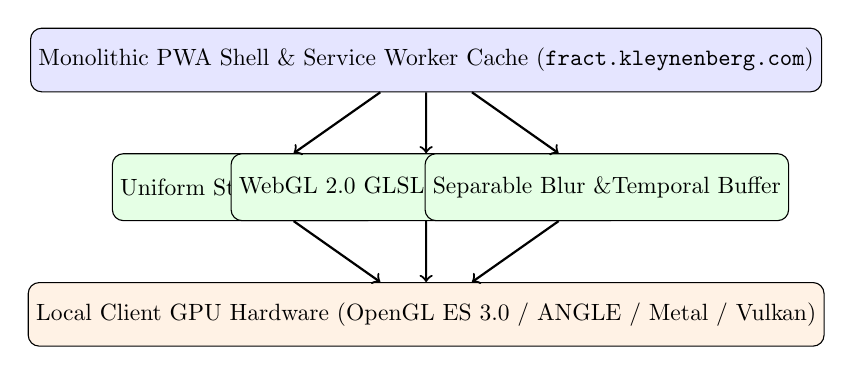
\begin{tikzpicture}[scale=0.85, every node/.style={scale=0.85}]
    \node[draw, rectangle, rounded corners, minimum width=7.6cm, minimum height=0.95cm, fill=blue!10] (pwa) at (0, 3.0) {Monolithic PWA Shell \& Service Worker Cache (\texttt{fract.kleynenberg.com})};
    \node[draw, rectangle, rounded corners, minimum width=2.3cm, minimum height=1.0cm, fill=green!10] (ui) at (-2.7, 1.1) {Uniform State\\Controller};
    \node[draw, rectangle, rounded corners, minimum width=2.5cm, minimum height=1.0cm, fill=green!10] (webgl) at (0.0, 1.1) {WebGL 2.0 GLSL\\Fragment Pipeline};
    \node[draw, rectangle, rounded corners, minimum width=2.3cm, minimum height=1.0cm, fill=green!10] (blur) at (2.7, 1.1) {Separable Blur \&\\Temporal Buffer};
    \node[draw, rectangle, rounded corners, minimum width=7.6cm, minimum height=0.95cm, fill=orange!10] (hw) at (0, -0.8) {Local Client GPU Hardware (OpenGL ES 3.0 / ANGLE / Metal / Vulkan)};

    \draw[->, thick] (pwa) -- (ui);
    \draw[->, thick] (pwa) -- (webgl);
    \draw[->, thick] (pwa) -- (blur);
    \draw[->, thick] (ui) -- (hw);
    \draw[->, thick] (webgl) -- (hw);
    \draw[->, thick] (blur) -- (hw);
\end{tikzpicture}
\caption{Data-flow architecture of the monolithic PWA runtime, isolating uniform state updates, WebGL 2.0 fragment computation, and temporal filtering directly on client GPU hardware.}
\label{fig:architecture}
\end{figure}

As illustrated in Figure~\ref{fig:architecture}, user pan/zoom gestures update lightweight uniform parameters while the WebGL 2.0 render loop evaluates the active fractal universe into an offscreen framebuffer object (FBO) before post-processing.

\subsection{Mathematical Formulation of the Three Fractal Universes}
\subsubsection{Universe 1: Perturbation-Theory Mandelbrot Set}
The quadratic Mandelbrot recurrence is defined for $c \in \mathbb{C}$ by:
\begin{equation}
z_{n+1} = z_n^2 + c, \quad z_0 = 0.
\end{equation}
To exceed single-precision floating-point zoom limits without full per-pixel multi-precision emulation, the viewport center $c_0$ is evaluated along a high-precision reference trajectory $\{z_n\}_{n=0}^{N_{\max}}$. Any neighboring pixel parameter $c = c_0 + \delta_c$ follows a perturbed trajectory $z_n + \delta_n$:
\begin{equation}
z_n + \delta_n = (z_{n-1} + \delta_{n-1})^2 + (c_0 + \delta_c),
\end{equation}
which simplifies to the variational recurrence~\cite{quilezfractal}:
\begin{equation}
\delta_{n+1} = 2 z_n \delta_n + \delta_n^2 + \delta_c, \quad \delta_0 = 0.
\end{equation}
Because $|\delta_n|$ and $|\delta_c|$ remain small relative to the zoom window prior to escape, every pixel shader evaluates $\delta_{n+1}$ in native 32-bit floating-point hardware while preserving deep-zoom structural fidelity.

\subsubsection{Universe 2: Transcendental Newton--Raphson Basins}
To render continuous attraction basins of non-polynomial complex maps, the second universe applies the generalized Newton--Raphson iteration:
\begin{equation}
z_{n+1} = z_n - \frac{f(z_n)}{f'(z_n)}.
\end{equation}
For the transcendental function $f(z) = z^3 - e^z \cos(z) - 1$, analytical differentiation yields the closed-form step:
\begin{equation}
z_{n+1} = z_n - \frac{z_n^3 - e^{z_n}\cos(z_n) - 1}{3z_n^2 - e^{z_n}(\cos(z_n) - \sin(z_n))}.
\end{equation}
Root basins are shaded by combining final root phase angles with smooth iteration-count damping.

\subsubsection{Universe 3: M\"obius-Transformed Apollonian Gaskets}
The third universe renders recursive inversive circle packings governed by Descartes' Circle Theorem. For four mutually tangent circles with signed curvatures $k_i = \pm 1/r_i$:
\begin{equation}
(k_1 + k_2 + k_3 + k_4)^2 = 2(k_1^2 + k_2^2 + k_3^2 + k_4^2).
\end{equation}
Continuous conformal motion across the complex plane is achieved by pre-transforming fragment coordinates through time-parameterized M\"obius transformations:
\begin{equation}
M(z) = \frac{az + b}{cz + d}, \quad ad - bc = 1, \quad a,b,c,d \in \mathbb{C},
\end{equation}
followed by iterative circle inversions into the fundamental Apollonian domain.

\subsection{Separable Sub-Pixel Blur and Velocity-Weighted Temporal Accumulation}
High-frequency fractal filaments exhibit severe spatial aliasing when sampled at one ray per pixel, whereas brute-force $K \times K$ supersampling multiplies fragment shader invocations by $K^2$. To suppress sub-pixel shimmer at linear cost, the post-processing pipeline applies a two-pass separable 1D Gaussian filter of radius $R$ over the raw FBO intensity $I(x,y)$:
\begin{equation}
I'(x,y) = \sum_{i=-R}^{R} I(x + i, y) \cdot \frac{1}{\sqrt{2\pi}\sigma} \exp\left(-\frac{i^2}{2\sigma^2}\right),
\end{equation}
followed by the orthogonal vertical pass. The spatially filtered frame is then blended with the reprojected previous accumulation buffer $C_{\text{prev}}(x',y')$ via a velocity-weighted exponential moving average:
\begin{equation}
C_{\text{final}}(x,y) = \alpha \, I''(x,y) + (1 - \alpha) \, C_{\text{prev}}(x',y'),
\end{equation}
with adaptive blend factor
\begin{equation}
\alpha = \min\left(1.0, \frac{1}{1 + \kappa \|\mathbf{v}\|}\right),
\end{equation}
where $\mathbf{v}$ denotes the instantaneous screen-space pan/zoom velocity vector and $\kappa > 0$ controls responsiveness. When the camera slows or halts ($\|\mathbf{v}\| \to 0$), $\alpha$ decreases to accumulate sub-pixel detail across frames; during rapid motion, $\alpha \to 1$ prevents ghosting trails.

\section{Complexity Analysis and Reference Verification}
\subsection{Asymptotic Computational and Memory Complexity}
For a viewport of resolution $W \times H$ pixels and maximum iteration depth $N_{\max}$, the worst-case per-frame arithmetic complexity of fragment evaluation is bounded by:
\begin{equation}
\mathcal{O}(W \cdot H \cdot N_{\max}),
\end{equation}
while the separable two-pass spatial filter adds $\mathcal{O}(W \cdot H \cdot R)$ texture lookups independent of $N_{\max}$. Under perturbation rendering, the high-precision reference orbit incurs $\mathcal{O}(N_{\max})$ scalar work once per camera anchor update, amortizing precision cost across all $W \cdot H$ parallel GPU fragments. Framebuffer memory footprint remains bounded by two RGBA FBO ping-pong targets of size $\mathcal{O}(W \cdot H)$, avoiding dynamic heap allocations during animation.

\subsection{Live Artifact Verification}
Rather than relying on static screenshots or synthetic offline traces, the complete monolithic PWA is deployed for direct empirical inspection on arbitrary desktop and mobile GPUs at \url{https://fract.kleynenberg.com/} and \url{https://fractinity.netlify.app/}. Users and automated evaluators can verify offline Service Worker persistence, real-time shader responsiveness, and sub-pixel temporal stabilization directly in any WebGL 2.0-capable browser.

\section{Discussion and Limitations}
Three practical boundaries govern browser-based fractal rendering:
\begin{enumerate}
    \item \textbf{Reference Orbit Glitches:} In perturbation rendering, if a pixel trajectory passes close to a minibrot center where $|z_n + \delta_n| \ll |z_n|$, catastrophic cancellation can occur in $\delta_n$, requiring glitch detection and secondary reference rebasing.
    \item \textbf{Browser Shader Compilation Variance:} Cross-platform translation layers (ANGLE on Chromium, Metal-backed WebGL on Safari) enforce distinct loop-unrolling and uniform-buffer limits, requiring bounded loop counters in GLSL ES 3.00.
    \item \textbf{Mobile Thermal and Fill-Rate Envelopes:} On battery-powered mobile GPUs, sustained high-$N_{\max}$ fragment execution at native high-DPI resolutions may trigger dynamic clock scaling unless adaptive resolution scaling is enabled.
\end{enumerate}

\section{Conclusion}
This paper presented a self-contained, zero-dependency monolithic PWA architecture for real-time fractal rendering in WebGL 2.0, exemplified by the live Fractinity application (\url{https://fract.kleynenberg.com/} and \url{https://fractinity.netlify.app/}). Combining perturbation theory for deep-zoom Mandelbrot evaluation, analytical Newton--Raphson and M\"obius--Apollonian formulations, and velocity-weighted temporal accumulation over separable Gaussian filters achieves smooth interactive exploration within standard browser sandboxes without external server infrastructure.

\begin{thebibliography}{10}

\bibitem{mandelbrot1982fractal}
B.~B. Mandelbrot, \emph{The Fractal Geometry of Nature}.\hskip 1em plus 0.5em minus 0.4em\relax New York, NY, USA: W. H. Freeman and Company, 1982.

\bibitem{peitgen1986beauty}
H.-O. Peitgen and P.~H. Richter, \emph{The Beauty of Fractals: Images of Complex Dynamical Systems}.\hskip 1em plus 0.5em minus 0.4em\relax Berlin, Germany: Springer-Verlag, 1986.

\bibitem{berriman2015pwa}
F.~Berriman and A.~Russell, ``Progressive Web Apps: Escaping tabs without losing our soul,'' \emph{Infrequently Noted}, Jun. 2015. \url{https://infrequently.org/2015/06/progressive-apps-escaping-tabs-without-losing-our-soul/}

\bibitem{khronoswebgl2}
The Khronos Group, \emph{WebGL 2.0 Specification}.\hskip 1em plus 0.5em minus 0.4em\relax Beaverton, OR, USA: Khronos Open Standard, 2023. \url{https://registry.khronos.org/webgl/specs/latest/2.0/}

\bibitem{parisi2012webgl}
T.~Parisi, \emph{WebGL: Up and Running}.\hskip 1em plus 0.5em minus 0.4em\relax Sebastopol, CA, USA: O'Reilly Media, 2012.

\bibitem{quilezfractal}
I.~Quilez, ``Perturbation theory and Mandelbrot rendering articles,'' \emph{Inigo Quilez Technical Articles}, 2024. \url{https://iquilezles.org/articles/mandelbrot/}

\bibitem{hennessy2011computer}
J.~L. Hennessy and D.~A. Patterson, \emph{Computer Architecture: A Quantitative Approach}, 5th~ed.\hskip 1em plus 0.5em minus 0.4em\relax Waltham, MA, USA: Morgan Kaufmann, 2011.

\end{thebibliography}

\end{document}
